\input{configuration}

\def\ojoin{\setbox0=\hbox{$\bowtie$}%
  \rule[-.02ex]{.25em}{.4pt}\llap{\rule[\ht0]{.25em}{.4pt}}}
\def\leftouterjoin{\mathbin{\ojoin\mkern-5.8mu\bowtie}}

\title{Tutorial 7 --- Data Mining and Transactions }

\author{Richard Wong \\ \small \texttt{rk2wong@edu.uwaterloo.ca}}
\institute{Department of Electrical and Computer Engineering \\
  University of Waterloo}
\date{\today}


\begin{document}

\begin{frame}
  \titlepage

\end{frame}


\begin{frame}
\frametitle{Exercise 7-1}

What is a data warehouse, and why is it useful to have one?

\end{frame}


\begin{frame}
\frametitle{Exercise 7-1 Solution}

What is a data warehouse, and why is it useful to have one?

\begin{itemize}
  \item Maintain OLTP responsiveness by having separate hardware handle OLAP queries
  \item A data warehouse can be optimized for read access
  \item Reshape (denormalize) OLTP schema into star/snowflake schema to simplify OLAP queries
  \item Star/snowflake schemas enable cubing operations on data (look up "OLAP cube")
  \item Most OLAP queries deal in aggregates, which could benefit from column-oriented storage
  \item and more...
\end{itemize}

\end{frame}


\begin{frame}
\frametitle{Exercise 7-2}

Suppose we are trying to predict the value \textit{Wait}. \\
Between attributes \textit{Pat} and \textit{Type}, which is better to split a decision node on?

\begin{center}
  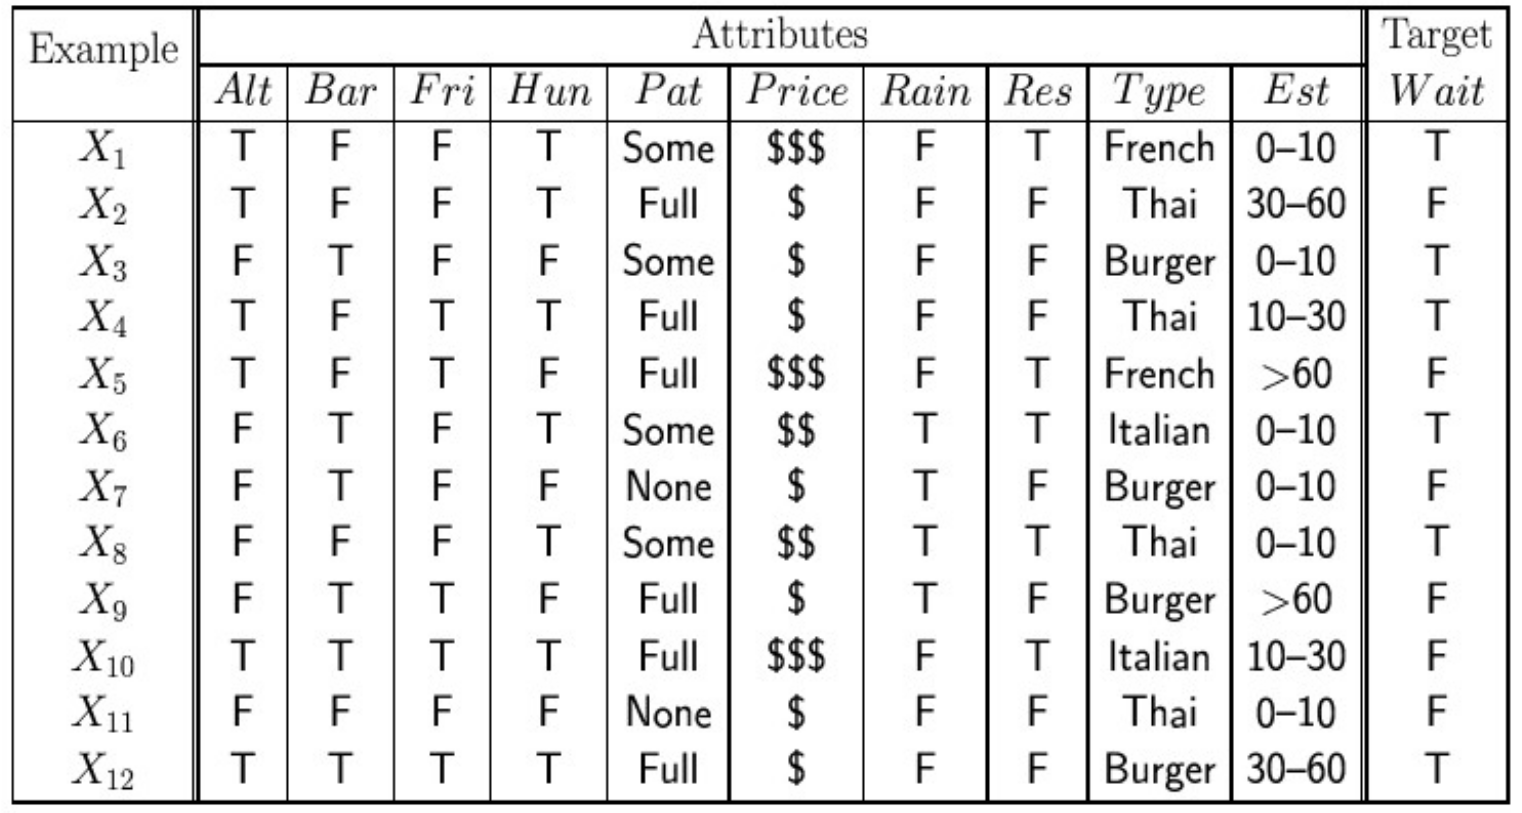
\includegraphics[width=0.9\textwidth]{images/decision_matrix.png}
\end{center}

\end{frame}


\begin{frame}
\frametitle{Exercise 7-2 Solution (1/3)}

Let's use entropy ($I$) as the metric that we want to minimize.

We have two choices of attributes (\textit{Pat} and \textit{Type}), and we want to pick the one that maximizes information gain. So first we should find out the entropy of the full data set $S$.

\begin{align*}
  I(S) &= -\sum_{i=1}^{\{T, F\}}p_i\log_2(p_i) \\
  &= -p_T\log_2(p_T) - p_F\log_2(p_F) \\
  &= -(\frac{6}{12})\log_2(\frac{6}{12}) - (\frac{6}{12})\log_2(\frac{6}{12}) \\
  &= -(\frac{1}{2})(-1) - (\frac{1}{2})(-1) \\
  &= \frac{1}{2} + \frac{1}{2} \\
  &= 1
\end{align*}

\end{frame}


\begin{frame}
\frametitle{Exercise 7-2 Solution (2/3)}

So $I(S) = 1$.

\begin{align*}
  I(S_{Pat}) &= P_{Pat=None}I(S_{Pat=None}) + P_{Pat=Some}I(S_{Pat=Some}) + P_{Pat=Full}I(S_{Pat=Full}) \\
  &= \frac{2}{12}(0) + \frac{4}{12}(0) + \frac{6}{12}I(S_{Pat=Full}) \\
  &= \frac{1}{2} (0.918) \\
  IG_{Pat} &= I(S) - I(S_{Pat}) \\
  &= 1 - \frac{1}{2} (0.918) \\
  &= 0.541
\end{align*}

\end{frame}


\begin{frame}
\frametitle{Exercise 7-2 Solution (3/3)}

\begin{align*}
  I(S_{Type}) &= P_{Type=French}I(S_{Type=French}) + P_{Type=Italian}I(S_{Type=Italian}) \\
  &+ P_{Type=Thai}I(S_{Type=Thai}) + P_{Type=Burger}I(S_{Type=Burger}) \\
  &= \frac{1}{4}(1) + \frac{1}{4}(1) + \frac{1}{4}(1) + \frac{1}{4}(1) \\
  &= 1 \\
  IG(S_{Type}) &= I(S) - I(S_{Type}) \\
  &= 1 - 1 \\
  &= 0
\end{align*}

So $IG(S_{Pat}) = 0.541$, $IG(S_{Type}) = 0$. \\
$IG(S_{Pat}) > IG(S_{Type})$, so $Pat$ is the better attribute to split on.

\end{frame}


\begin{frame}
\frametitle{Exercise 7-3}

What are the ACID transaction properties, and what can a database do to ensure each one?

\end{frame}


\begin{frame}
\frametitle{Exercise 7-3 Solution (1/2)}

The ACID properties:

\begin{itemize}
  \item Atomicity: the effects of a transaction either fully take place, or none at all.
  \item Consistency preservation: the state of a database before and after a transaction is consistent.
  \item Isolation: transactions can operate unaware of concurrent transactions.
  \item Durability: transaction completion guarantees persistence (i.e. write to disk or stable storage, backup, etc.)
\end{itemize}

\end{frame}


\begin{frame}
\frametitle{Exercise 7-3 Solution (2/2)}

How do we ensure each one?

\begin{itemize}
  \item Atomicity: keep a sequential log of each task that executes in a transaction. Each log entry should contain sufficient data to roll back. In addition, only allow execution of recoverable transaction schedules.
  \item Consistency: abort transactions that would violate constraints.
  \item Isolation: this can be done to varying degrees. It is up to the transaction manager to uphold isolation guarantees, which the DBA may decide on.
  \item Durability: never report that a transaction is committed until it is persisted.
\end{itemize}

\end{frame}


\begin{frame}
\frametitle{Exercise 7-4}

Distinguish between the following:

\begin{enumerate}
  \item a serial schedule
  \item a serializable schedule
  \item a conflict-serializable schedule
\end{enumerate}

\end{frame}


\begin{frame}
\frametitle{Exercise 7-4 Solution}

\begin{enumerate}
  \item serial: aside from the first transaction in the schedule, each transaction only starts after the previous has committed.
  \item serializble: the schedule is \textit{equivalent} to a serial schedule using the same transactions, for some definition of \textit{equivalent}.
  \item conflict-serializable: the schedule is \textit{conflict-equivalent} to a serial schedule using the same transactions.
\end{enumerate}

If you can swap two consecutive \textit{non-conflicting} operations (belonging to different transactions) in a schedule, then the schedules before and after the swap are considered to be \textit{conflict-equivalent}. \\
Two operations are \textit{conflicting} iff at least one of them is a write, and they both operate on the same data.

\end{frame}


\begin{frame}
\frametitle{Exercise 7-5}

Is the following schedule conflict-serializable? \\
If not, how can we make it conflict-serializable?

\begin{center}
\begin{tabular}{ c c c c c c c }
  \hline
  T1 & r(x) & & w(y) & & & \\
  \hline
  T2 & & r(y) & & & r(x) & \\
  \hline
  T3 & & & & w(x) & & r(x) \\
  \hline
\end{tabular}
\end{center}

\end{frame}


\begin{frame}
\frametitle{Exercise 7-5 Solution}

\begin{center}
\begin{tabular}{ c c c c c c c }
  \hline
  T1 & r(x) & & w(y) & & & \\
  \hline
  T2 & & r(y) & & & r(x) & \\
  \hline
  T3 & & & & w(x) & & r(x) \\
  \hline
\end{tabular}
\end{center}

This schedule is not conflict-serializable. To show that there is no sequence of transformations that can take the given schedule to a serial schedule, we use the concept of a precedence graph.

In this graph, we create a \textit{node for each transaction}, then proceed to add edges.

A directed edge from transaction X to transaction Y in the precedence graph means that \textit{X precedes Y}. That means that whatever serial schedule we come up with needs to execute everything in X befor everything in Y.

We add an edge from X to Y where an operation in X occurs before and conflicts with an operation in Y.

A cycle in the precedence graph means that no serial ordering of the transactions will be conflict-equivalent with the given schedule. Try creating the graph as an exercise.

To make the schedule conflict-serializable, remove nodes (i.e. abort transactions) until there are no cycles.

\end{frame}
\end{document}
